\begin{figure}[btp]
\subcapcentertrue
\subfigure[Single centralized DB]{
  \includegraphics[width=.3\linewidth]{figures/KVS-validation-G5K-SINGLEDB.png}
  \label{fig:exp-deployment-db}}
\subfigure[REDIS Key/Value Store]{
  \includegraphics[width=.3\linewidth]{figures/KVS-validation-G5K-REDIS.png}
  \label{fig:exp-deployment-redis}}
\subfigure[Galera]{
  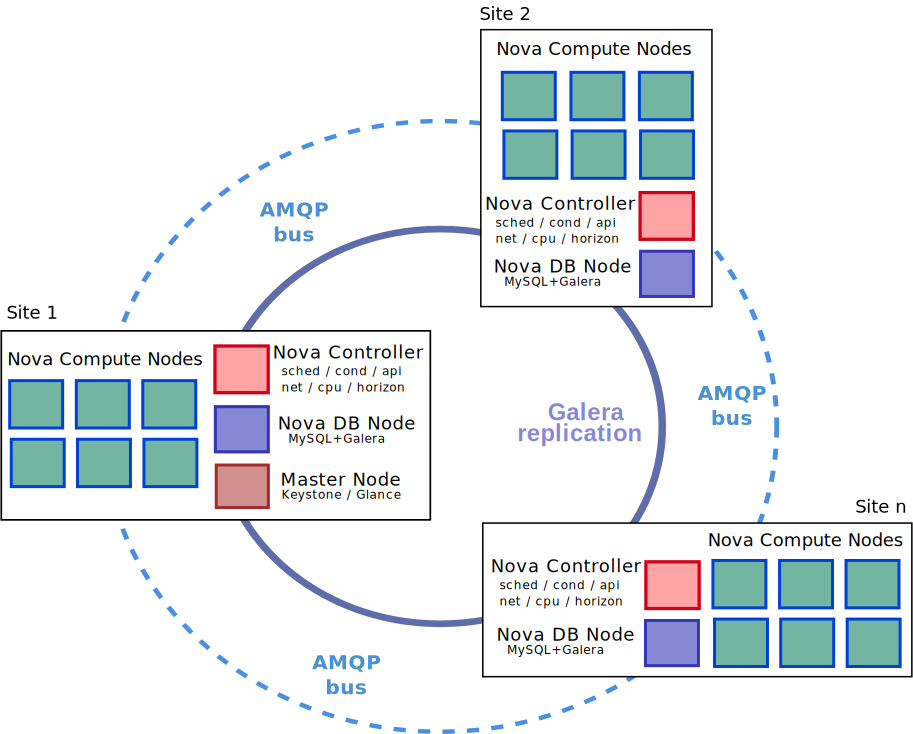
\includegraphics[width=.3\linewidth]{figures/KVS-validation-G5K-GALERA.png}
  \label{fig:exp-deployment-galera}}
\caption{Investigated deployments on top of G5K and role of each server node.}
\label{fig:exp-deployment}
%\vspace*{-.3cm}
\end{figure}


%%%
\section{Experimental Validation\label{sec:eval}}

The validation of our proof-of-concept has been done via three sets of
experiments. The first one aimed at measuring the impact of the use of the REDIS
NoSQL solution instead of the MySQL system in a single site deployment. The
second set focused on multi-site scenarios by comparing the impact of the
latency on our distributed Nova service with respect to an active/active Galera
deployment. Finally, the last experiment showed that higher level OpenStack mechanisms
are not impacted by the use of the REDIS KVS.

All Experiments have been performed on Grid'5000~\cite{grid5000}, a large-scale
and versatile experimental testbed that enables researchers to get an access to
a large amount of computing resources %(\(\sim\)
%1000 nodes spread over 10 sites)
with a very fine control of the experimental conditions. We deployed and
configured each node involved in the experiment with a customized software stack
(Ubuntu 14.04, a modified version of OpenStack ``Devstack'', and REDIS v3) using
Python scripts and the Execo toolbox~\cite{imbert:hal-00861886}. We underline
that we used the legacy network mechanisms integrated in Nova (\ie, without
Neutron) and deployed other components that were mandatory to perform our
experiment (in particular Keystone and Glance) on a dedicated node belonging to
the first site (entitled master node on Figure \ref{fig:exp-deployment}).

%%%
\subsection{Impact of REDIS w.r.t MySQL\label{subsec:monosite_experiments}}

\subsubsection{Time penalties}
Changes made over Nova's source code to support a NoSQL database as REDIS is
likely to affect its reactivity. The first reason is that a KVS does
not provide a support of operations like joining, and thus the code we developed
to provide such operations, creates a computation overhead. The second reason is
related to networking. Unlike a single MySQL node, in a REDIS system data is
spread over several nodes. Thus, a request can lead to several network
exchanges. Finally, REDIS provides a replication strategy to deal with fault
tolerant aspects, leading also to possible overheads.

\begin{table}[htb]
\centering
  \caption{\label{tab:orgtable3}
    Average response time to API requests for a mono-site deployment (in ms).}
\begin{tabular}{lrl}
Backend configuration & REDIS & MySQL\\
\hline
1 node & 83 & 37\\
4 nodes & 82 & -\\
4 nodes + repl & 91 & -\\
\end{tabular}
\end{table}


%% \begin{table}[htb]
%% \caption{\label{tab:orgtable0}
%% Time used to create 500 VMs on a single cluster configuration (in sec.)}
%% \centering
%% \begin{tabular}{rr}
%% REDIS & MySQL\\
%% \hline
%% 298 & 357\\
%% \end{tabular}
%% \end{table}


\begin{figure}[htbp]
  \centering

 % \vspace*{-.3cm}
      \includegraphics[width=.9\linewidth]{figures/cumulative_frequency_all_mysql1_redis1.png}
        \caption{Statistical distribution of Nova API response time (in ms.).}
        \label{fig:cumulated_frequency_api}
 %       \vspace*{-.3cm}
\end{figure}



\begin{table}[htb]
\centering
\caption{\label{tab:orgtable0}Time used to create 500 VMs on a single cluster configuration (in sec.)}
\begin{tabular}{lrl}
Backend configuration & REDIS & MySQL\\
\hline
1 node & 322 & 298\\
4 nodes & 327 & -\\
4 nodes + repl & 413 & -\\
\end{tabular}
\end{table}

%%%
\begin{figure*}[htp]
\subcapcentertrue
\subfigure[Single centralized DB]{
  \includegraphics[width=.30\linewidth]{figures/iftop_in_cumulative_sqlalchemy_2_1_10_True_1_False.png}
  \label{fig:network_bar_mysql_1}}
\subfigure[4 nodes REDIS cluster without replication]{
  \includegraphics[width=.30\linewidth]{figures/iftop_in_cumulative_redis_2_1_10_False_4_False.png}
  \label{fig:network_bar_redis_4_norepl}}
\subfigure[4 nodes REDIS cluster with replication (1 replica)]{
  \includegraphics[width=.30\linewidth]{figures/iftop_in_cumulative_redis_2_1_10_True_4_False.png}
  \label{fig:network_bar_redis_4_repl}}
\caption{Amount of data exchanged per type of nodes, varying the DB configuration (MySQL or  REDIS).}
\label{fig:data_exchanged}
%\vspace*{-.3cm}
\end{figure*}


Table~\ref{tab:orgtable3} compares average response times used to satisfy API
requests made during the creation of 500 VMs on an infrastructure deployed over
one cluster (containing 1 controller node and 6 compute nodes), using either
REDIS or the MySQL backend under the three aforementioned scenarios. While the
distribution of REDIS between several nodes and the use of the replication
feature do not significantly increase the response time (first column), the
difference between the average API response time of our KVS approach and the
vanilla MySQL code may look critical at first sight (124\% higher). However, it
must be mitigated with Figure~\ref{fig:cumulated_frequency_api} and
Table~\ref{tab:orgtable0}.
%Leveraging data from experiments of the first line of Table~\ref{tab:orgtable3},
Figure~\ref{fig:cumulated_frequency_api} depicts the statistical distribution of
the response time of each API call that has been made during the creation of the
500 VMs. It is noticeable that for a large part of them (around 80\%), our Rome/REDIS
solution delivers better performance than the SQLAlchemy/MySQL backend.
%Exactly, 75\% of the API calls are processed in less than 40ms while MySQL needs 59ms.
On the other side, the 10\% of the slowest API calls are above 222~ms with our
proposal while they are are around 86~ms when using MySQL. Such a difference
explains the averages recorded in Table~\ref{tab:orgtable3} and we need to
conduct deeper investigations to identify the kind of requests and how they can
be handled in a more effective way. Overall, we can see that even with these
slow-requests, the completion time for the creation of 500 VMs is competitive as
illustrated by Table ~\ref{tab:orgtable0}. In other words, some API
functions have a more significant impact than others on the VM creation time.

%% Indeed as indicated above, this overhead mainly comes from the
%% computation overhead to map SQL requests with a noSQL backend. The second line
%% of Table~\ref{tab:orgtable3} illustrates that distributing the key/value store
%% on several nodes creates an overhead related to networking (in our case, data is
%% distributed over four nodes). This overhead represents 1\% of what is measured
%% with the single node key/value store, which means that there is little or no
%% cost associated with distributed a key/value database on few nodes. The third
%% line represents measurements with data replication enabled. The overhead is then
%% less than 11\% compared to a clustered configuration without replication. This
%% small overhead can be obtained thanks to the asynchronous strategy used in
%% REDIS. Globally, the average response time is 146\% slower than was has been
%% initially measured with a single MySQL node.

%% As some API  functions have a more significant impact  than others on the
%% VM creation time, according to the  first lines of Table \ref{tab:orgtable3} and
%% Table \ref{tab:orgtable0}, data of these two  tables cannot be correlated in the
%% case of  two different database, while  according the ``REDIS'' columns  of both
%% Table  \ref{tab:orgtable3} and  Table \ref{tab:orgtable0}  indicates that  for a
%% given database type, a corellation can be made.

\subsubsection{Networking penalties}

As we target the deployment of an OpenStack infrastructure over a large number of geographical sites linked together through the Internet backbone,
the quantity of data exchanged is an important criterion for the evalution of our solution. In particular, as data is stored in the KVS with an object
structure, it requires a serialization/deserialization phase when objects are stored/queried.  To enable this serialization, the addition of some
metadata is required, which leads to a larger data footprint and thus a larger amount of data exchanged between database nodes and OpenStack nodes.

To determine wether the level of network-overhead is acceptable or not,
networking data has been collected during the previous experiments. Table
\ref{tab:data_exchanged_comparison} compares the total amount of data exchanged
over network depending of the database configuration that has been used. As
MySQL does not store serialized objects, \ie objects are serialized at the
client-side by the ORM, thus only raw data is exchanged over the network, we
consider the single node MySQL as the optimal solution, which has been measured
at 1794MB. Our solution deployed over a single REDIS node consumes 2190MB, which
means that the networking overhead related to the combination of ROME and REDIS
is estimated to be around 22\%. Doing the same experiment with a 4 nodes REDIS
cluster without data replication leads to a 33\% networking overhead compared to
a single MySQL node. Finally, when the data replication is enabled with one
replica, the amount of data exchanged over the network is 76\% higher than
without replication, which is intuitive.

However, the infrastructures that have been deployed contain
different kind of nodes (controllers, compute nodes, database nodes, ...) and
the aforementioned data takes everything into account and thus it does not
enable us to get a precise view of the origin of the networking overhead.

\begin{table}[htb]
\caption{\label{tab:data_exchanged_comparison} Amount of data exchanged over the
  network (in MBytes)} \centering
\begin{tabular}{lrl}
Backend configuration & REDIS & MySQL\\
\hline
1 node & 2190 & 1794 \\
4 nodes & 2382 & -\\
4 nodes + repl (1 replica) & 4186 & -\\
\end{tabular}
\end{table}

By using the \textbf{iftop}~\footnote{http://www.ex-parrot.com/pdw/iftop/} tool,
it has been possible to gather information about the origin and destination of
TCP/IP messages exchanged during the creation of VMs, and thus to get a precise
idea of the origin of any networking overhead. Figure \ref{fig:data_exchanged}
depicts the data exchanges in function of the origin (horizontal axis) and the
destination (vertical bars), varying the database configuration. It is
noticeable that there is no significant difference in terms of exchange pattern
for OpenStack nodes, regardless the kind of nodes and regardless the DB
configuration that has been used (either MySQL or REDIS). We can notice slightly
different patterns for DB Nodes: a comparison of Figure
\ref{fig:network_bar_mysql_1} and \ref{fig:network_bar_redis_4_norepl} confirms
that the networking overhead depicted in Table
\ref{tab:data_exchanged_comparison} comes from the DB nodes. Finally,
Figure \ref{fig:network_bar_redis_4_repl} confirms that most of
the overhead observed when enabling data replication is also caused by additional
data exchanged between database nodes.

%%%
\subsection{Multi-site Scenarios\label{sec:multisite_exps}}

The second experiment we performed consisted in evaluating a single OpenStack deployment over several locations. Our goal was to compare the behaviour of a
single MySQL OpenStack with the advised Galera solution and our Rome+REDIS proposal. Figure~\ref{fig:exp-deployment} depicts how the nodes have been
configured for each scenario. While the deployment of a single MySQL node is a non sense in a production infrastructure as discussed before,
evaluating such a scenario enabled us to to get an indication regarding the maximum performance we can expect. Indeed in such a scenario, the DB is
deployed on a single server located in one of the locations, without any synchronization mechanism and consequently no overhead related to
communications with remote DB nodes on the contrary to a clustered Redis or an infrastructure composed of several MySQL DBs that are synchronized with
the Galera mechanism. Moreover, conducting such an experiment at large scale enabled us to see the limit of such a centralized approach.

%(\ie the an OpenStack
%infrastructure deployed over a single node relational database and then a
%clustered relational database were compared with the same kind of infrastructure
%distributed on top of a clustered REDIS database.

Regarding the experimental methodology, all executions have been conducted on
servers of the same site (Rennes) in order to ensure reproducibility:
\emph{distinct locations} (\ie clusters) have been emulated by adding latency
between group of servers thanks to the \texttt{TC} unix tool. Each
\emph{cluster} was containing 1 controller node, 6 compute nodes, and one DB
node when needed. Scenarios including 2, 4, 6, and 8 clusters have been
evaluated, leading to infrastructures composed of up to 8 controllers and 48
compute nodes overall. The latency between each cluster has been set to 10~ms
and then 50~ms. Finally, in order to evaluate the capability of such
infrastructures to distribute the workload on several controllers, and to detect
concurrency problems inherent in using a non relational DB backend, the creation
of the 500 VMs has been fairly distributed among the available controllers in
parallel.

\begin{table}[htb]
\caption{\label{tab:orgtable1}
Time to create 500 VMs with a 10ms inter-site latency (in sec.).}
\centering
\begin{tabular}{lrrr}
Nb of locations & REDIS & MySQL & Galera\\
\hline
2 clusters & 271 & 209 & 2199\\
4 clusters & 263 & 139 & 2011\\
6 clusters & 229 & 123 & 1811\\
8 clusters & 223 & 422 & 1988\\
\end{tabular}
\end{table}

\begin{table}[htb]
\caption{\label{tab:orgtable2}
Time to create 500 VMs with a 50ms inter-site latency (in sec.).}
\centering
\begin{tabular}{lrrl}
Nb of locations & REDIS & MySQL & Galera\\
\hline
2 clusters & 723 & 268 & *\\
4 clusters & 427 & 203 & *\\
6 clusters & 341 & 184 & -\\
8 clusters & 302 & 759 & -\\
\end{tabular}
\end{table}

Table~\ref{tab:orgtable1} and Table~\ref{tab:orgtable2} present the time to create the 500~VMs. As expected, increasing the number of clusters leads
to a decrease of the completion time.  This is explained by the fact that a larger number of clusters means a larger number of controllers and compute
nodes to handle the workload.

%This confirms that %increasing the number of controllers and compute nodes in
%an OpenStack leads to a better reactivity.

%% The results measured for  a 10ms latency, show that our  approach takes a rather
%% constant time to create 500 VMs, which stabilizes around 220 seconds. While such
%% a time is approximately twice the one  of the simple MySQL approach, it is eight
%% times better than the Galera advised solution.

%% The results measured for  a 10ms latency, show that our  approach takes a rather
%% constant time to create 500 VMs, which stabilizes around 260 seconds. While such
%% a time is approximately twice the one  of the simple MySQL approach, it is eight
%% times better than the Galera advised solution.

The results measured for a 10ms latency, show that our approach takes a rather constant time to create 500 VMs, which stabilizes around 220
seconds. While a single MySQL node has better results until 6 clusters, one can see the limitations of a single server with 8 clusters. In such a
case, the single MySQL performs 89\% slower than our approach, while the advised Galera solution is 891\% slower than our approach.

With a 50ms inter-cluster latency, the difference between REDIS and MySQL is accentuated in the 8 clusters configuration, as MySQL is 151\% slower
than our REDIS approach.
%
%
%% While the  \textit{MySQL} column in Table
%% \ref{tab:orgtable1} and  Table \ref{tab:orgtable2} suggests that  using a single
%% node  MySQL  provides better  results  than  REDIS,  these  results have  to  be
%% mitigated  with  the problem  of  not  being  fault-tolerant, unlike  the  REDIS
%% cluster. The  comparison of results  collected with  a REDIS cluster  with those
%% measured  in the  case of  a  clusterized MySQL  (with Galera),  shows that  our
%% approach   is  embarassingly   faster  than   the  one   advised  by   OpenStack
%% documentation:  in  a four  clusters  configuration  with a  10ms  inter-cluster
%
%

Regarding Galera, it is noteworthy that important issues related to concurrent modifications of the databases appear with a 50~ms latency, preventing
many of the 500~VMs to be created (\ie several bugs occur leading Nova to consider many VMs as crashed). Such pathological behaviours are due to
both the important latency between clusters and the burst mode we used to create the 500 VMs (for information, we succeeded to create 500 VMs but in a
sequential manner for 2 and 4 clusters).

To summarize, in addition to tackling the distribution issue, the couple
Rome+REDIS enables OpenStack to be scalable: the more controllers are taking
part to the deployment, the better the performance is.
%%%
\subsection{Compatibility with Advanced Features\label{sec:host_aggregates_exps}}

The third experiment aimed at validating the correct behaviour of existing
OpenStack mechanisms while using our Rome+REDIS solution. Indeed, in order to
minimize the intrusion in the OpenStack source code, modifications have been
limited to the \textbf{nova.db.api} component. This component can be considered
as the part of Nova that has the most direct interaction with the DB. Limiting
the modification to the source code of this component should enable us to
preserve compatibility with existing mechanisms at higher level of the stack. To
empirically validate such an assumption, we conducted experiments involving
multi-site and the usage of host-aggregate/availability-zone mechanism (one
advanced mechanism of OpenStack that enables the segregation of the
infrastructure). As with aforementioned experiments, our scenario
involved the creation of 500 VMs in parallel on a multi-sites OpenStack
infrastructure deployed on top of Rome+REDIS with data replication activated
(the replica factor was set to 1). Two sets of experiments were conducted: a set
where each node of a same geographical site was member of a same host aggregate (that is the same availability zone) and a second set of experiments involving flat multi-site
OpenStack (\ie without defining any availability zone). 

%% Table~\ref{tab:experiments_host_aggregates} compares time taken to create the
%% 500 VMs by switching from a flat deployment to a deployment based on
%% host-aggregates, and by varying the number of geographical sites. It is
%% noticeable that using host-aggregates in Rome+REDIS does not cause any problem
%% to OpenStack, even when increasing the number of geographical sites and thus the
%% replication effort caused by the latency. Comparing these results with the
%% results presented in Table~\ref{tab:orgtable1} clearly shows that these last
%% experiments are slower. We explain this situation by the fact that, in the
%% experiments presented in Table \ref{tab:orgtable1}, data replication was
%% disabled and database nodes were not disturbed by any invasive
%% network-monitoring tools as in these sets of experiments.


%% \begin{table}[htb]
%% \vspace{-0.5cm}
%% \caption{\label{tab:experiments_host_aggregates}
%% Time to create 500 VMs with a 10ms inter-site latency (in sec.) and using Redis with and without host-aggregates.}
%% \centering
%% \begin{tabular}{lrrr}
%% Nb of locations & With  & Without \\
%% \hline
%% 4 clusters & 582 & 532\\
%% 8 clusters & 492 & 588\\
%% \end{tabular}
%% \end{table}

Experimental  results show  that the  host-aggregate/availability-zone mechanism
behaves  correctly on  top of  our proposal.  While VMs  are correctly  balanced
according to  the locations where  they have  been started, the  flat multi-site
deployment led to a non uniform distribution with respectively 26\%, 20\%, 22\%,
32\% of the created VMs for a 4 clusters experiments.
